\documentclass[main.tex]{subfiles}
\begin{document}

\section{Plugins}

\subsection{Design of Plugins}

Plugin is the law in the DARC Protocol, and all programs and operations within DARC must adhere to the restrictions imposed by all plugins. For an individual plugin, it follows the logic outlined in the pseudo code below:

\begin{verbatim}
if plugin.condition:
    return plugin.returnType
\end{verbatim}

For the DARC protocol, the main difference between before-operation plugins and after-operation plugins lies in their return types. For before-operation plugins, as they determine whether a certain operation should be executed directly, rejected outright, or entered into a sandbox, they have three distinct return types that serve as their final decisions:

\begin{enumerate}
    \item \texttt{NO}. When the condition of a before-operation plugin is triggered, the plugin's decision for that operation is \texttt{NO}. This decision indicates that the plugin believes the operation violates its rules, and therefore, it is rejected outright before entering the sandbox for execution.

    \item \texttt{SANDBOX\_NEEDED}. When the condition of a before-operation plugin is triggered, the plugin's decision for that operation is \texttt{SANDBOX\_NEEDED}. This decision indicates that the plugin cannot determine whether the operation should be accepted or rejected. The plugin is aware that the operation needs to be evaluated in the sandbox by after-operation plugins, and thus, the decision is made to let the operation proceed to the sandbox for further evaluation.

    \item \texttt{YES\_AND\_SKIP\_SANDBOX}. When the condition of a before-operation plugin is triggered, the plugin's decision for that operation is \texttt{YES\_AND\_SKIP\_SANDBOX}. This decision indicates that the plugin has determined that the operation should be approved and does not require execution in the sandbox. Therefore, the operation can proceed directly without going through the sandbox.
\end{enumerate}



For after-operation plugins, since the program has been executed in the sandbox and voting can commence, these plugins can have three return types as their final decisions:

\begin{enumerate}
    \item \texttt{NO}. When the condition of an after-operation plugin is triggered, the plugin's decision for the operation is \texttt{NO}. This decision indicates that the plugin believes the operation violates its rules and should be rejected outright.

    \item \texttt{VOTING\_NEEDED}. When the condition of an after-operation plugin is triggered, the plugin's decision for the operation is {VOTING\_NEEDED}. This decision indicates that the plugin believes the operation requires a vote, and the operation needs to initialize a voting item based on the voting rule specified by this plugin.

    \item \texttt{YES}. When the condition of an after-operation plugin is triggered, the plugin's decision for the operation is \texttt{YES}. This decision indicates that the plugin believes, based on its rules, the operation should be allowed to proceed.
\end{enumerate}


Each plugin has a condition node array, where condition nodes are stored in sequence. The root node corresponds to the node at index 0, which is the first node. The condition node array follows the following principles:

\begin{enumerate}
    \item The type of each node can be a boolean operator or an expression;
    \item For boolean operators, the type must be set as one of AND, OR, or NOT;
    \item For AND and OR operators, at least two valid child node indices must be specified in the child node list;
    \item For the NOT operator, a unique child node index must be specified in the child node list;
    \item For expression nodes, valid condition expression parameters consistent with the expression must be set;
    \item For expression nodes, the length of their child node list must be 0, meaning no child nodes are allowed.
\end{enumerate}

Figure \ref{fig:condition-nodes} is an example illustrating how a condition expression binary tree is serialized into a condition node array.

\begin{figure}
\centering
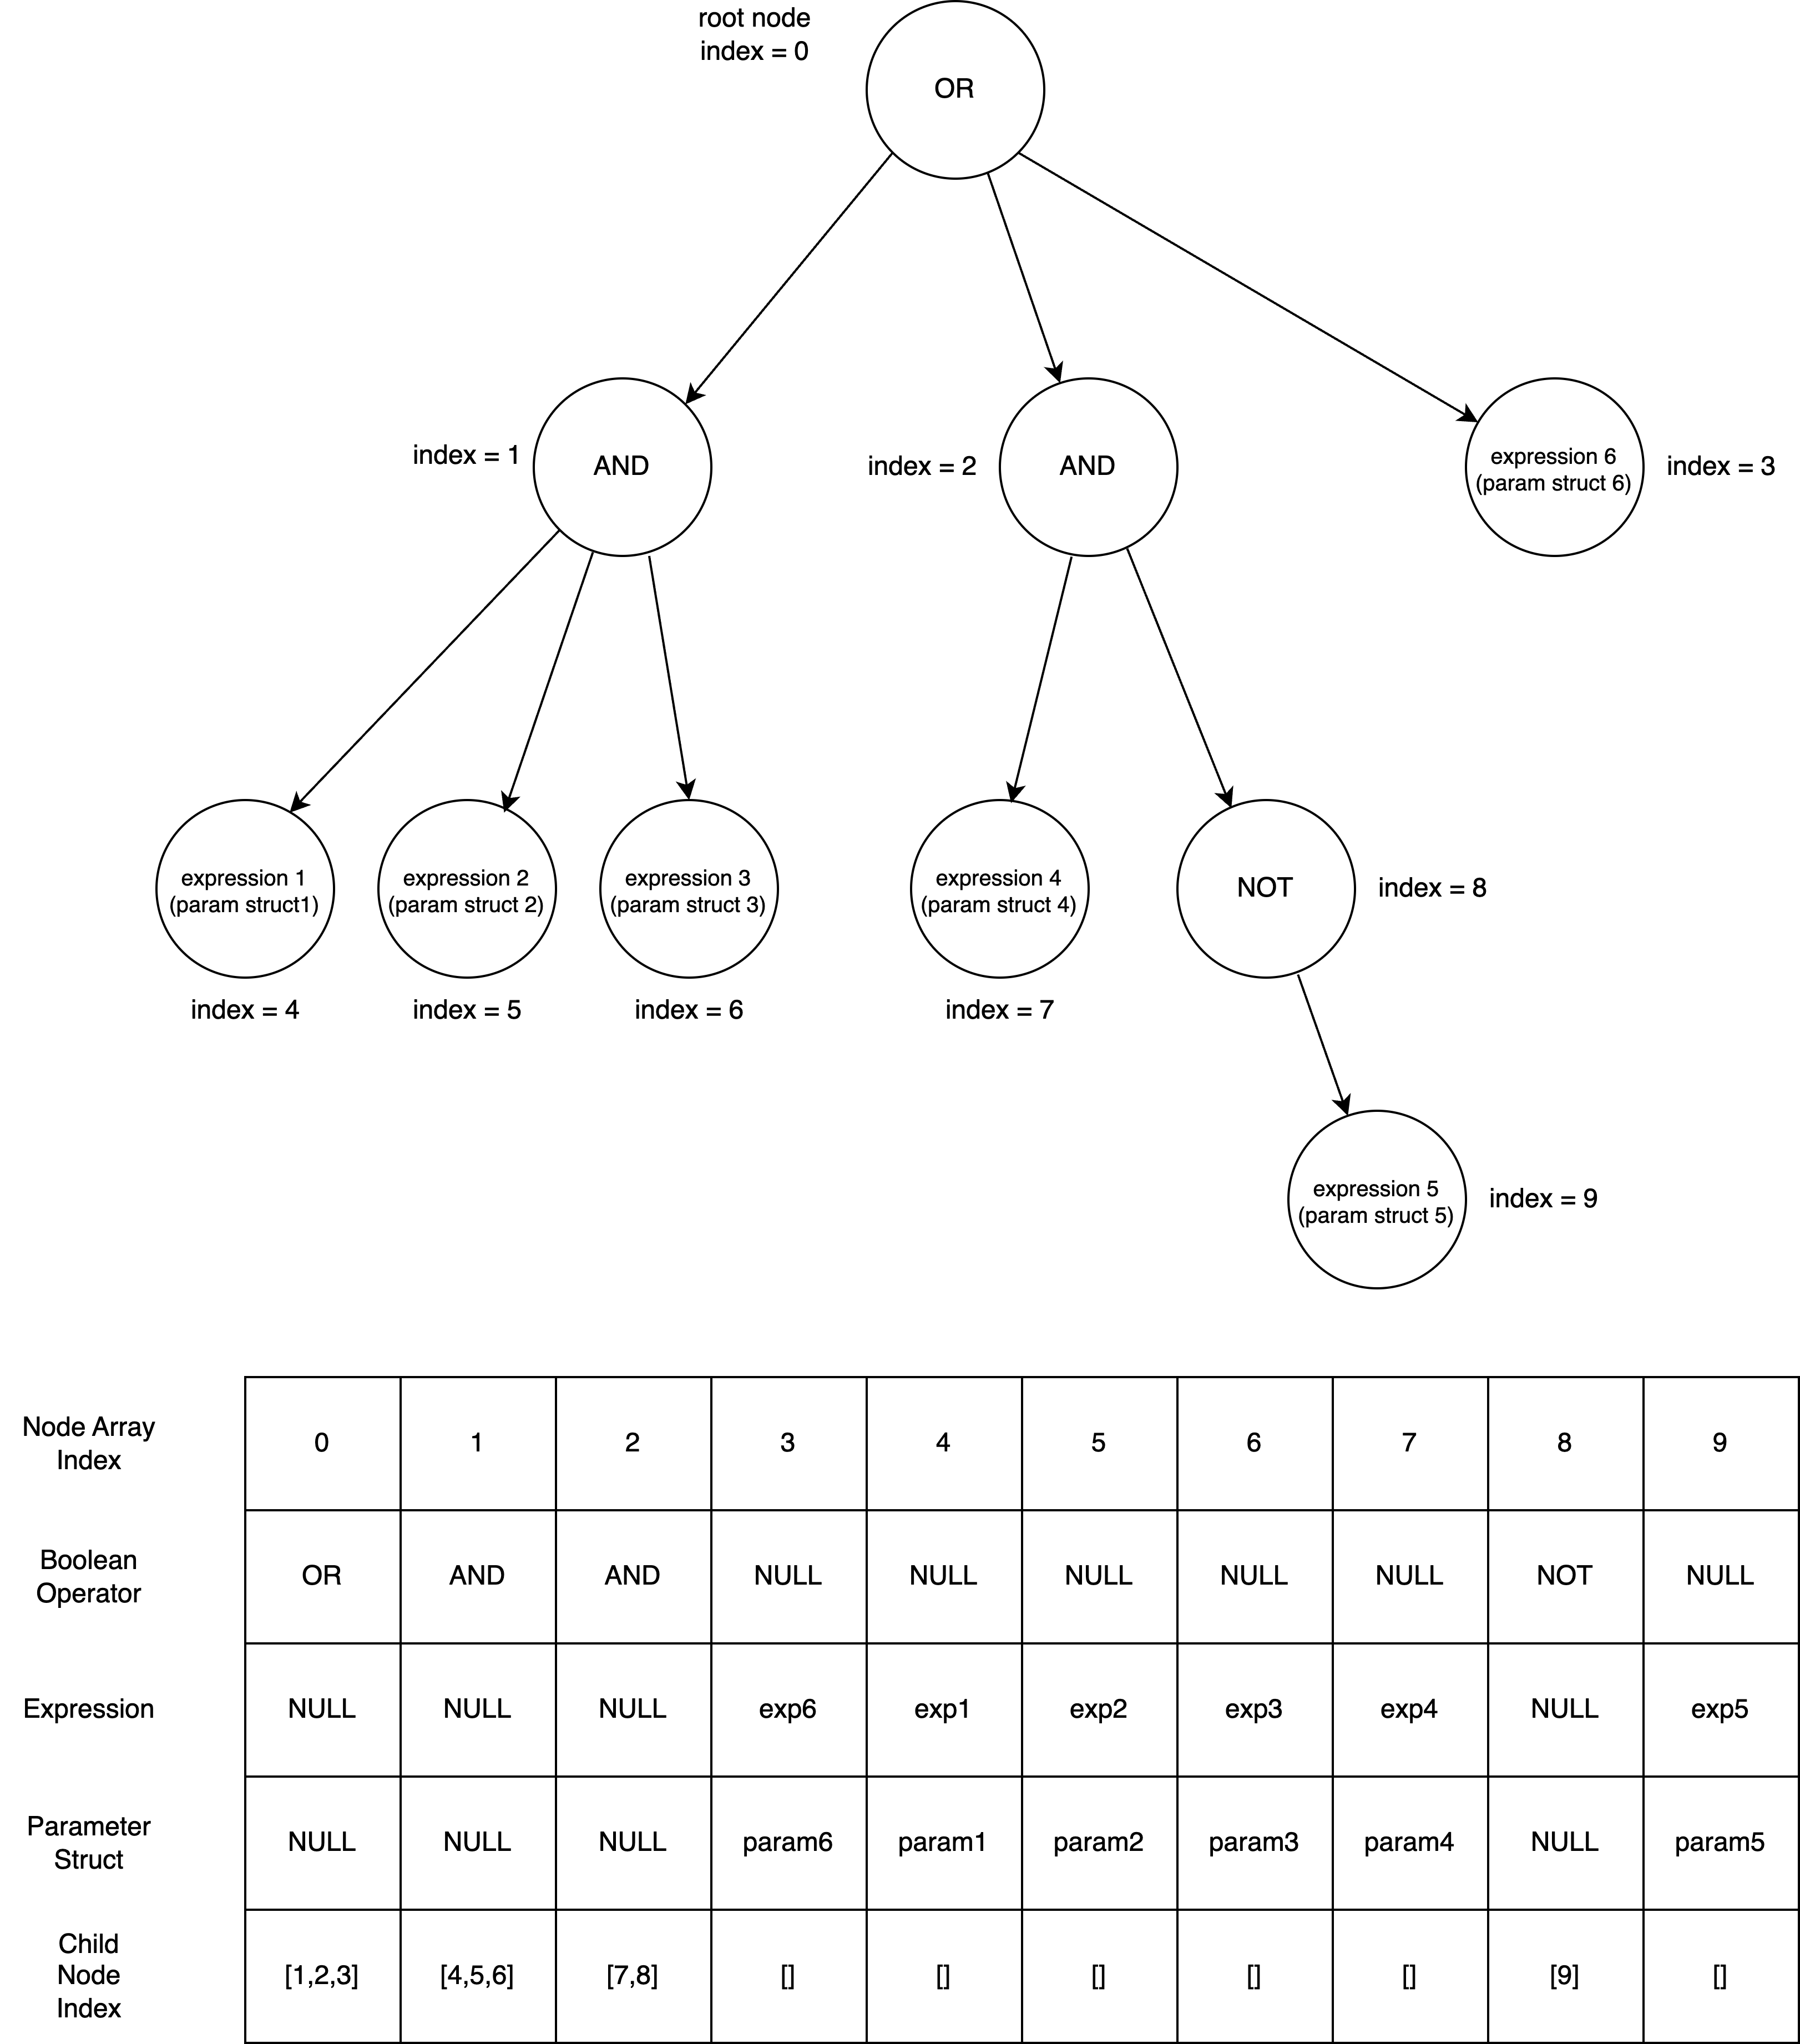
\includegraphics[width=1\linewidth]{plugin_condition_nodes.drawio.png}
\caption{\label{fig:condition-nodes}Condition Nodes and Expression Tree}
\end{figure}

Additionally, a plugin needs to set two parameters: one is the ``level'', representing the priority of the plugin within the entire plugin system. For the same operation, the judgment system traverses all plugins, and it is possible that at least two or more plugins are triggered. In such cases, if the levels of the plugins are different, the judgment system will consider the plugin with the higher level as the final determination.

The other parameter is the ``voting rule index'', which points to a specific index in the voting rule array. When the final decision of a plugin is \texttt{VOTING\_NEEDED}, the plugin requests the DARC protocol to use the voting rule indicated by the voting rule index for initializing the voting item. If the return type of the plugin is not \texttt{VOTING\_NEEDED}, the voting rule index will be ignored.



\subsection{Plugins and the Judgement System}

For the DARC protocol, the judgment system needs to undergo two assessments: one through before-operation plugins and another after the program has run completely in the sandbox, followed by evaluation through after-operation plugins. The reason for this design is that, without a sandbox and relying solely on a set of plugins for judgment, it becomes challenging to anticipate the behavior of the program. As a result, it is not possible to protect against modifications to special states in the DARC protocol.

For example, in a DARC instance where shareholder X is required to permanently hold 15\% voting rights and 10\% dividend rights, when designing a plugin, it is impossible to predict the state of the DARC instance after the execution of operations like mint tokens or burn tokens. This uncertainty poses challenges in ensuring that shareholder X maintains permanent ownership of 15\% voting rights and 10\% dividend rights. Only by running the operation in the sandbox and then re-evaluating the state of the sandbox, can such modifications be prevented.

In another scenario, if there is a need to ensure that a DARC instance reserves 10000 native tokens permanently before January 1, 2035, the correct detection and prevention of operations such as paying dividends or withdrawing cash can only be guaranteed by executing these operations in the sandbox. After all operations are completed in the sandbox, the judgment system performs a second evaluation through after-operation plugins. Without a sandbox and relying solely on plugins, the design of such a mechanism would be overly complex.


If there are only after-operation plugins and a sandbox without before-operation plugins, it would be expensive and inefficient. This is because the running cost of the sandbox is very high. It not only requires the program to run completely in the sandbox but also involves initializing the sandbox by fully replicating the internal state of the entire DARC instance. This process incurs a significant amount of gas fees.

For the majority of simple operations that can be approved without the need for running in the sandbox, it is more cost-effective to have rules established directly in before-operation plugins. For example, the trading of shares between small shareholders and retail investors, customers engaging in daily transactions, board members executing routine payment operations, and employees issuing salaries and stock incentives to themselves—these numerous daily and high-frequency activities can be defined as before-operation plugins. This approach helps to save gas fees for the vast majority of daily operations.



For before-operation plugins, whenever a program is submitted to the DARC protocol, the judgment system sequentially checks each operation. For each operation, the judgment system traverses each before-operation plugin and obtains a single judgment result. Finally, it aggregates the results for all operations to determine the overall result for the entire program. This decision dictates whether the program needs to run in the sandbox (\texttt{SANDBOX\_NEEDED}), be rejected outright (\texttt{NO}), or run directly without the need for the sandbox (\texttt{YES\_AND\_SKIP\_SANDBOX}). For before-operation judgment, the following rules are followed:

\begin{enumerate}
    \item If any operation is judged by the judgment system as \texttt{NO}, the entire program is rejected with a result of \texttt{NO}.
    \item If none of the operations is judged by the judgment system as \texttt{NO}, and at least one operation is judged as \texttt{SANDBOX\_NEEDED}, the entire program is required to run in the sandbox, and the result is \texttt{SANDBOX\_NEEDED}.
    \item If all operations are judged by the judgment system as \texttt{YES\_AND\_SKIP\_SANDBOX}, the entire program is approved with a result of \texttt{YES\_AND\_SKIP\_SANDBOX}, the entire program can skip the sandbox.
\end{enumerate}




\begin{figure}
\centering
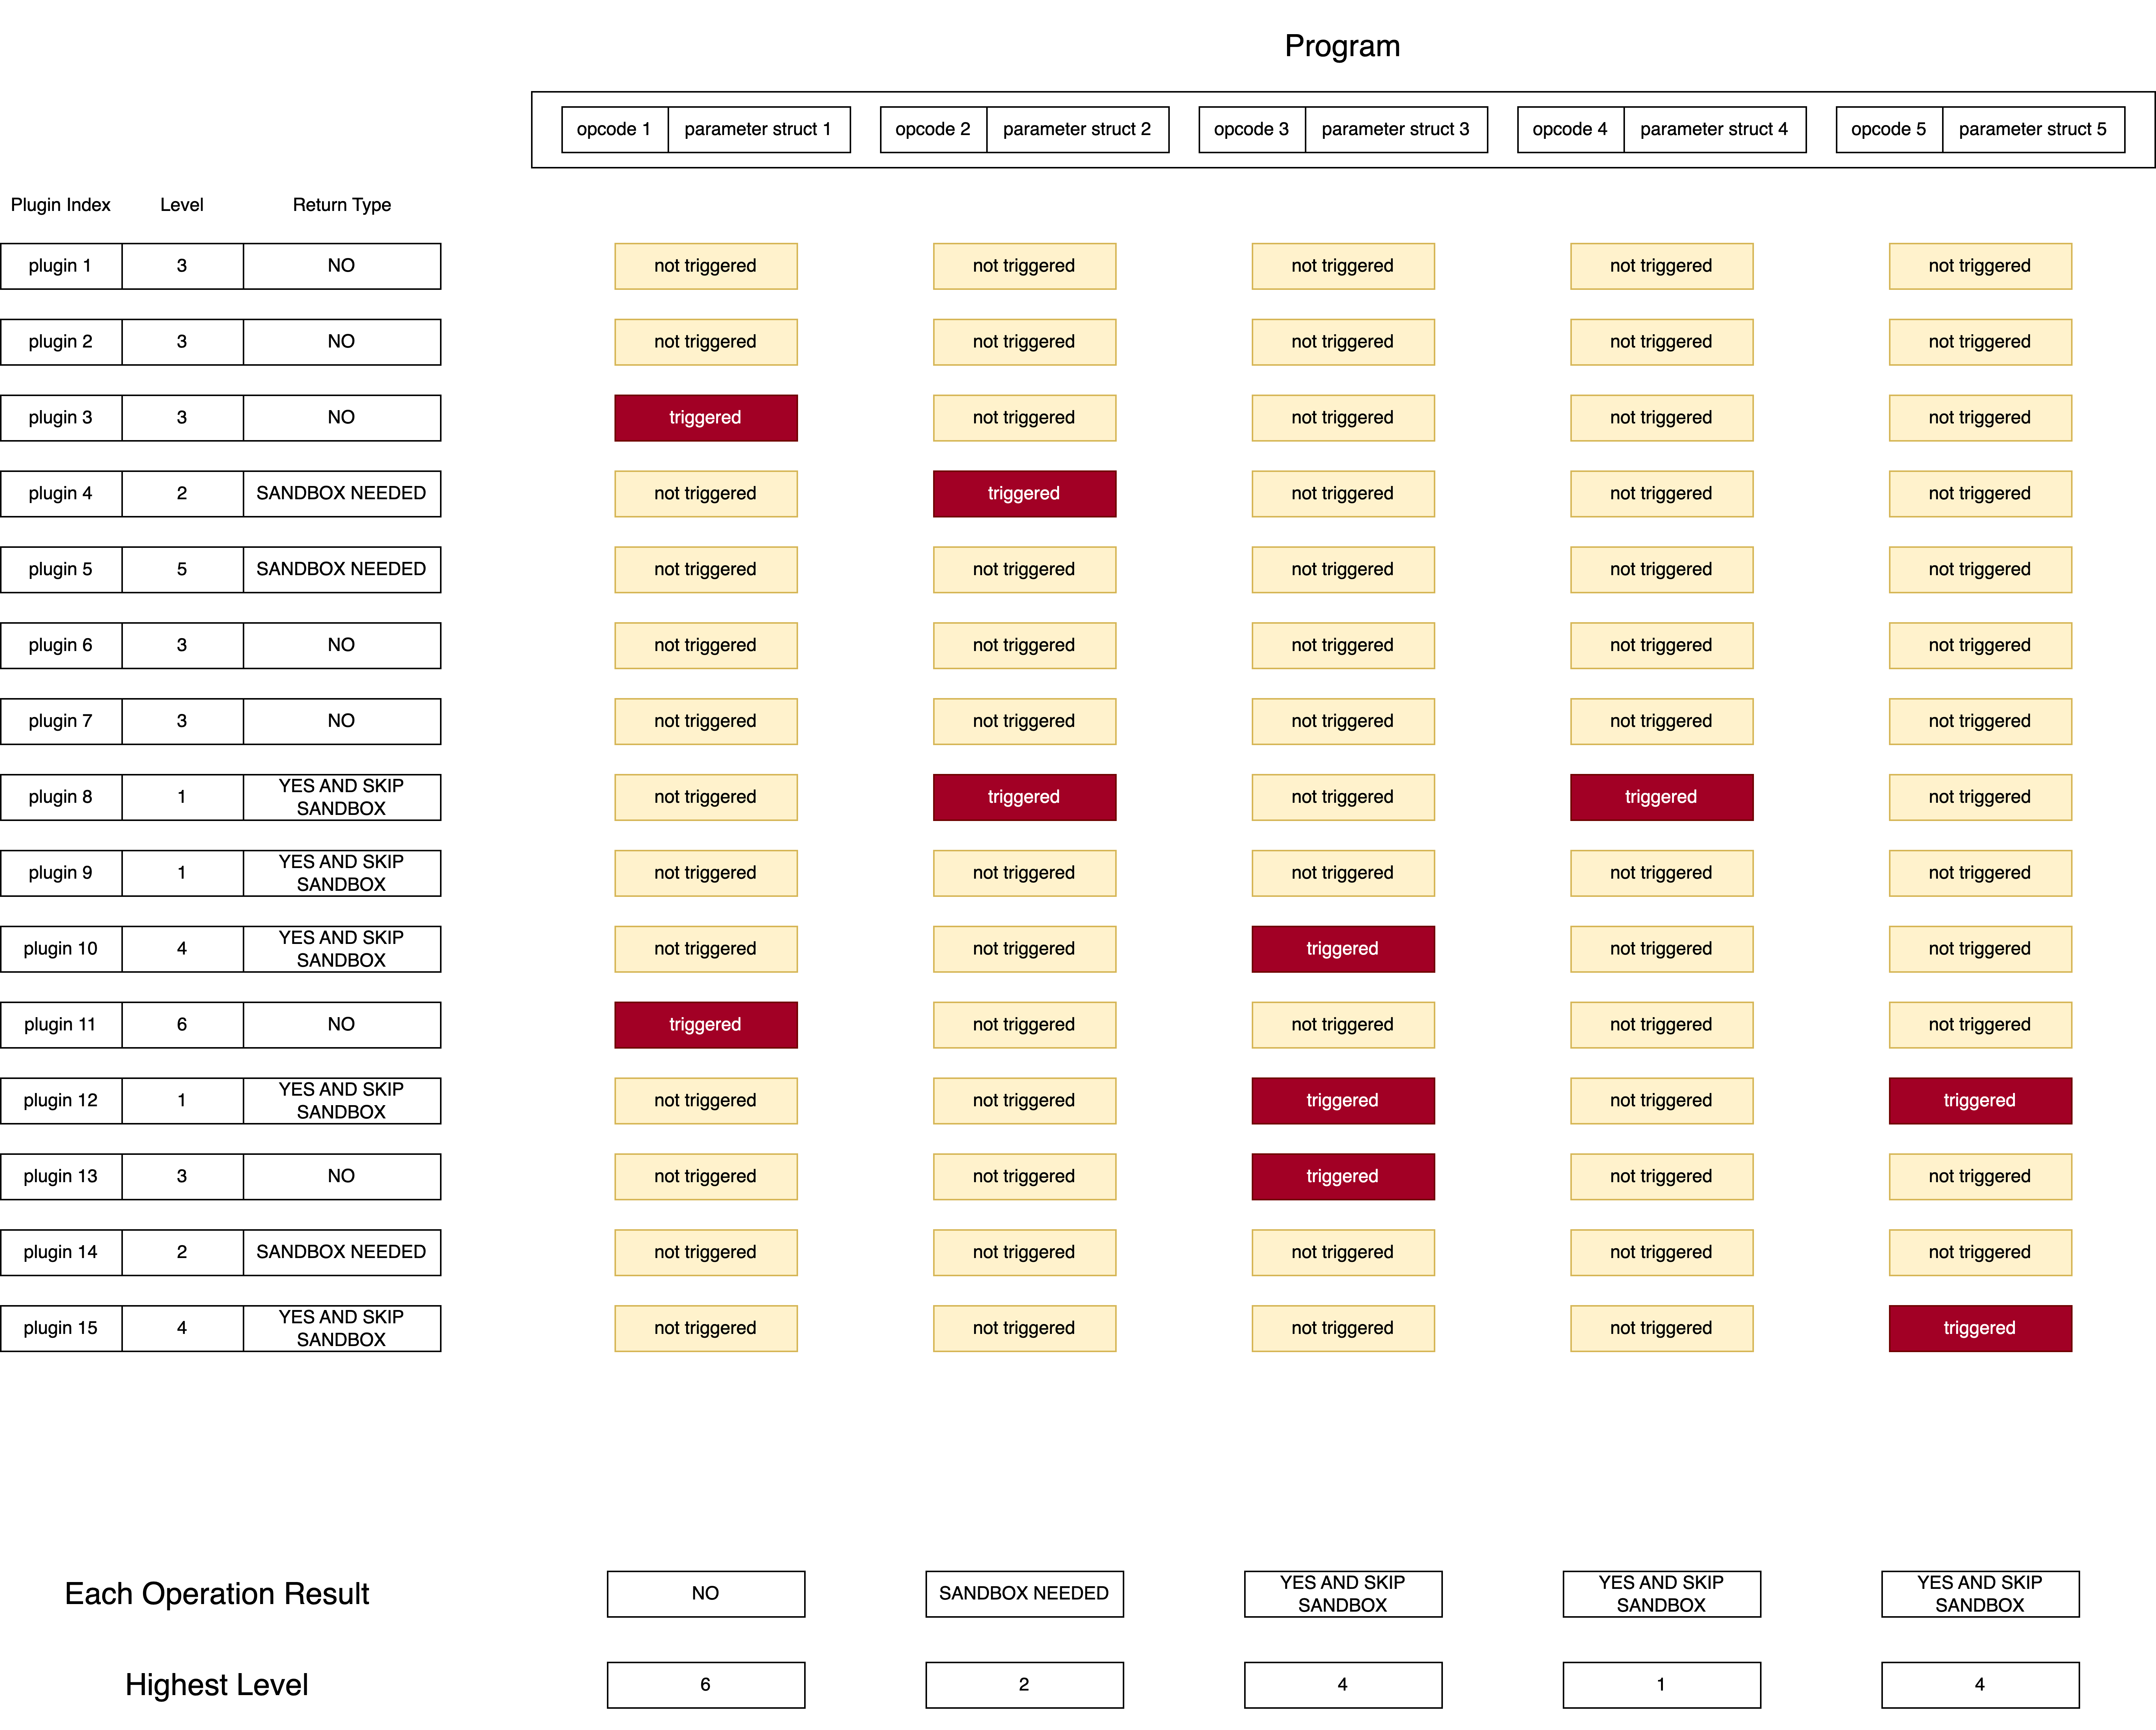
\includegraphics[width=1\linewidth]{judgement_plugin_levels_before_ops.drawio.png}
\caption{\label{fig:judgement-before-op}Judgement on program with before-operation plugins}
\end{figure}


Figure \ref{fig:judgement-before-op} illustrates how individual operations within a program are judged by before-operation plugins, resulting in judgment outcomes, deciding whether the program needs approval through voting (\texttt{VOTING\_NEEDED}), should be rejected outright (\texttt{NO}), or can proceed directly (\texttt{YES}). The following rules apply to after-operation judgment:

\begin{enumerate}
    \item If any operation is judged by the judgment system as \texttt{NO}, the entire program is rejected with a result of \texttt{NO}.
    \item If none of the operations have been determined as \texttt{NO} by the judgement system, and at least one operation has been determined as \texttt{VOTING\_NEEDED}, the final judgement for the entire program is \texttt{VOTING\_NEEDED}. This program will be placed into the pending program category, and the DARC protocol must initiate the voting system to decide on approval or rejection.
    \item If all operations are judged by the judgment system as \texttt{YES}, the entire program is approved with a result of \texttt{YES}, the entire program can be executed directly.
\end{enumerate}


\begin{figure}
    \centering
    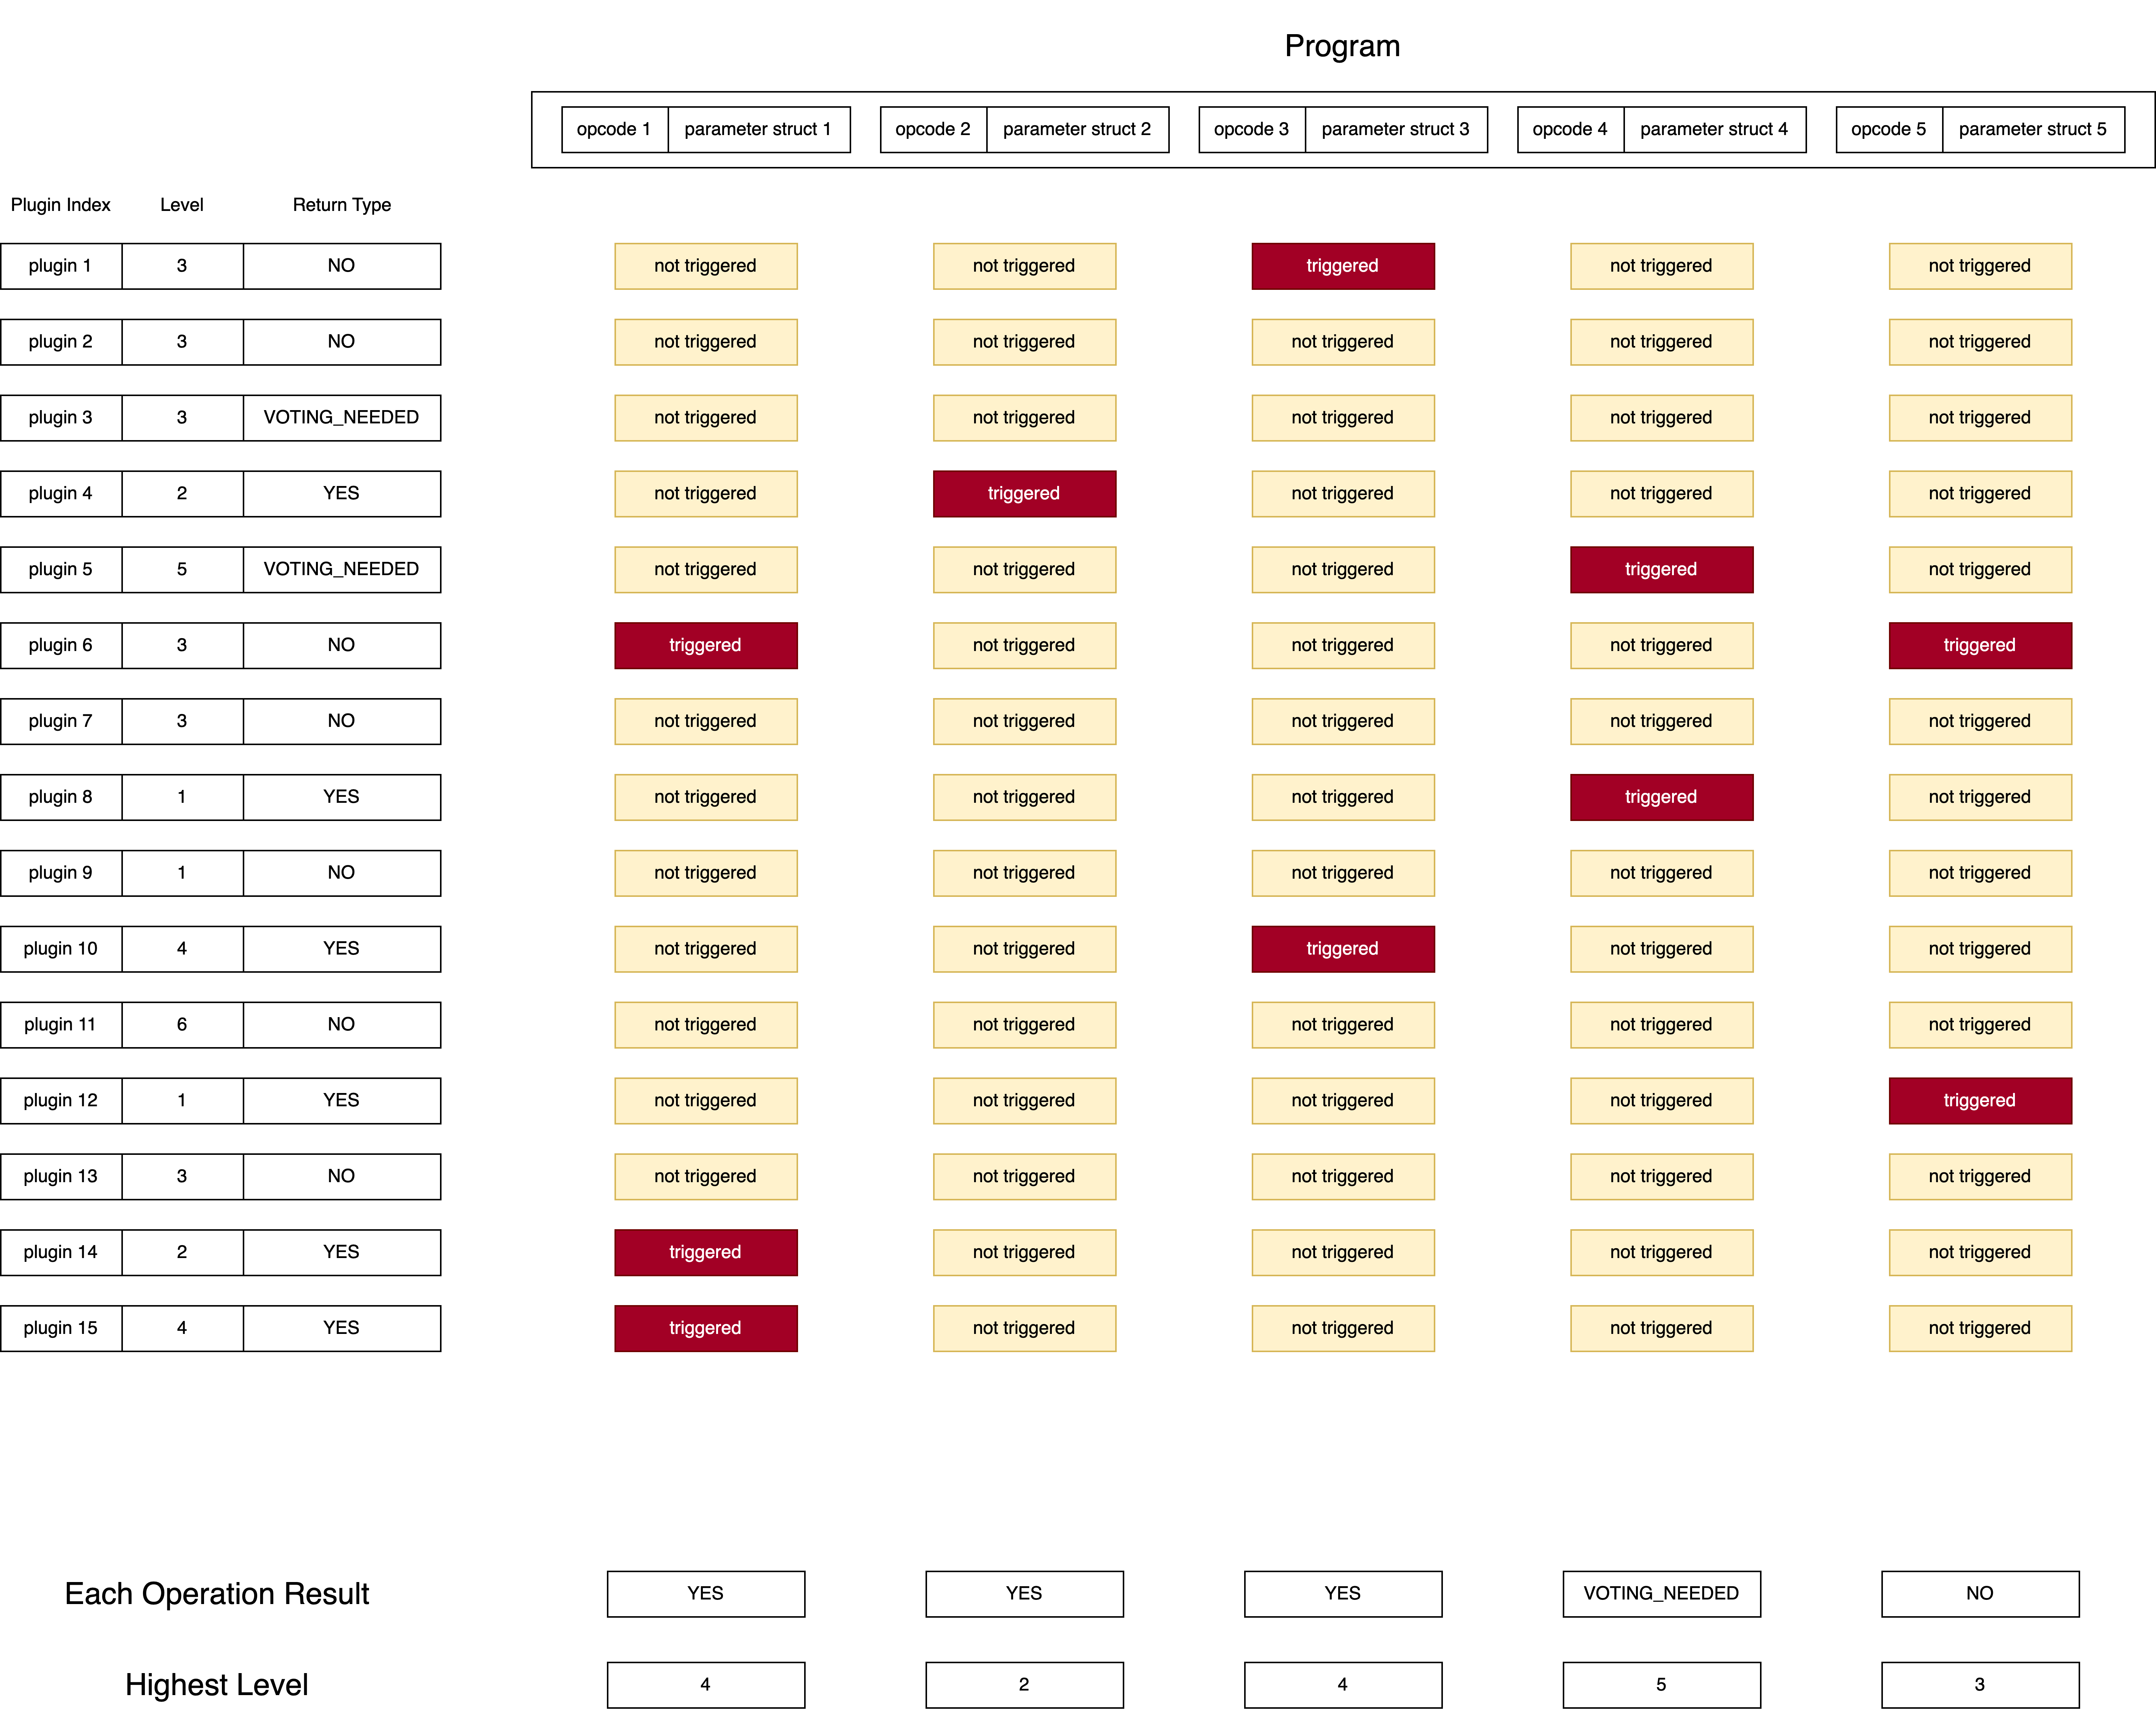
\includegraphics[width=1\linewidth]{judgement_plugin_levels_after_ops.drawio.png}
    \caption{\label{fig:judgement-after-op}Judgement on program with after-operation plugins}
\end{figure}

Figure \ref{fig:judgement-after-op} illustrates how individual operations within a program are judged by after-operation plugins, resulting in judgment outcomes.



\end{document}